\documentclass[noinstructornotes]{ximera}
%handout:  for handout version with no solutions or instructor notes
%handout,instructornotes:  for instructor version with just problems and notes, no solutions
%noinstructornotes:  shows only problem and solutions

%% handout
%% space
%% newpage
%% numbers
%% nooutcomes

%I added the commands here so that I would't have to keep looking them up
%\newcommand{\RR}{\mathbb R}
%\renewcommand{\d}{\,d}
%\newcommand{\dd}[2][]{\frac{d #1}{d #2}}
%\renewcommand{\l}{\ell}
%\newcommand{\ddx}{\frac{d}{dx}}
%\everymath{\displaystyle}
%\newcommand{\dfn}{\textbf}
%\newcommand{\eval}[1]{\bigg[ #1 \bigg]}

%\begin{image}
%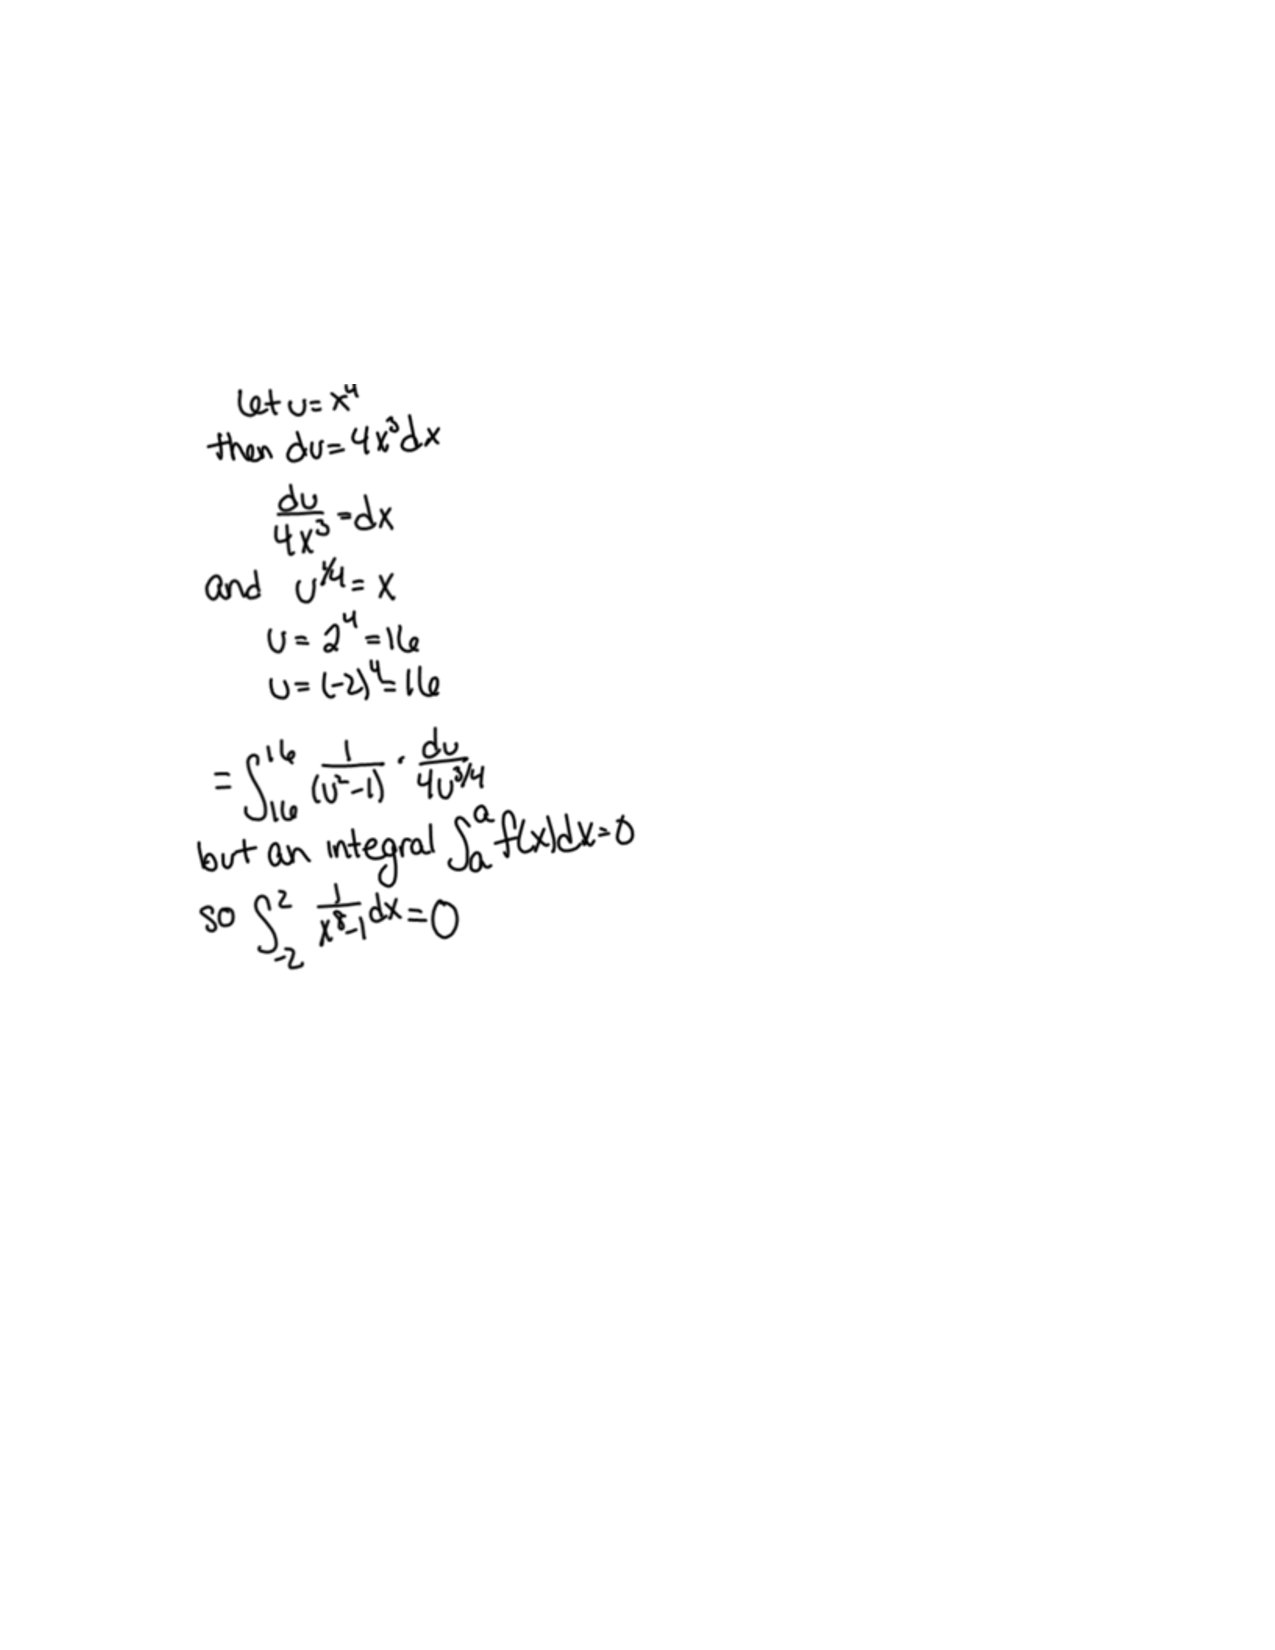
\includegraphics[trim= 170 420 250 180]{Figure1.pdf}
%\end{image}

%add a ``.'' below when used in a specific directory.
\newcommand{\RR}{\mathbb R}
\renewcommand{\d}{\,d}
\newcommand{\dd}[2][]{\frac{d #1}{d #2}}
\renewcommand{\l}{\ell}
\newcommand{\ddx}{\frac{d}{dx}}
\newcommand{\dfn}{\textbf}
\newcommand{\eval}[1]{\bigg[ #1 \bigg]}

\usepackage{multicol}

\renewenvironment{freeResponse}{
\ifhandout\setbox0\vbox\bgroup\else
\begin{trivlist}\item[\hskip \labelsep\bfseries Solution:\hspace{2ex}]
\fi}
{\ifhandout\egroup\else
\end{trivlist}
\fi} %% we can turn off input when making a master document

\title{Recitation \# 4: Volume by Shells}  

\begin{document}
\begin{abstract}		\end{abstract}
\maketitle




\section{Warm up:}
%problem 1
\begin{problem}
Determine whether you should integrate in terms of $x$ or $y$ in the given scenarios:
\begin{itemize}

	\item[(a)] You are revolving around the $y$-axis and using shells.
	
	\begin{freeResponse}
	If you are revolving around the $y$-axis, then the axis is vertical.  If you are using shells, the slices should be parallel to the axis so they should also be vertical.  Therefore, you should integrate in terms of $x$.
	\end{freeResponse}
	
	\item[(b)] You are revolving around $y=2$ and using washers.

	\begin{freeResponse}
	If you are revolving around the line $y=2$, then your axis is horizontal.  If you are using washers, the slices should be perpendicular to the axis.  Thus, the slices should be vertical.  Thus, you should integrate in terms of $x$.
	\end{freeResponse}

\end{itemize}


\end{problem}

%problem 2
	
	\begin{problem}
Determine whether you should use washers or shells:
\begin{itemize}

	\item[(a)] You are revolving around $x=3$ and want to integrate in terms of $y$.

	\begin{freeResponse}
	If you are revolving around $x=3$, then the axis is vertical.  If you want to integrate in terms of $y$, then you will have horizontal slices.  Therefore, your slices will be perpendicular to the axis.  Thus, you must use washers.
	\end{freeResponse}
	
	\item[(b)] You are revolving around the $x$-axis and want to integrate in terms of $y$.

	\begin{freeResponse}
	If you are revolving around the $x$-axis, the axis is horizontal.  If you want to integrate in terms of $y$, then you will have horizontal slices.  Therefore, your slices will be parallel to the axis.  Thus, you must use shells.
	\end{freeResponse}

\end{itemize}


\end{problem}
	
\begin{instructorNotes}

\end{instructorNotes}








\section{Group work:}


%problem 3
\begin{problem}
Consider the region bounded by $y=2-2x$, $y=2$, and $x=1$.  Use both the washer and shell method to find the volume of the solid formed by revolving this region around $y=-1$.  Do your answers match?


	\begin{freeResponse}
\begin{image}
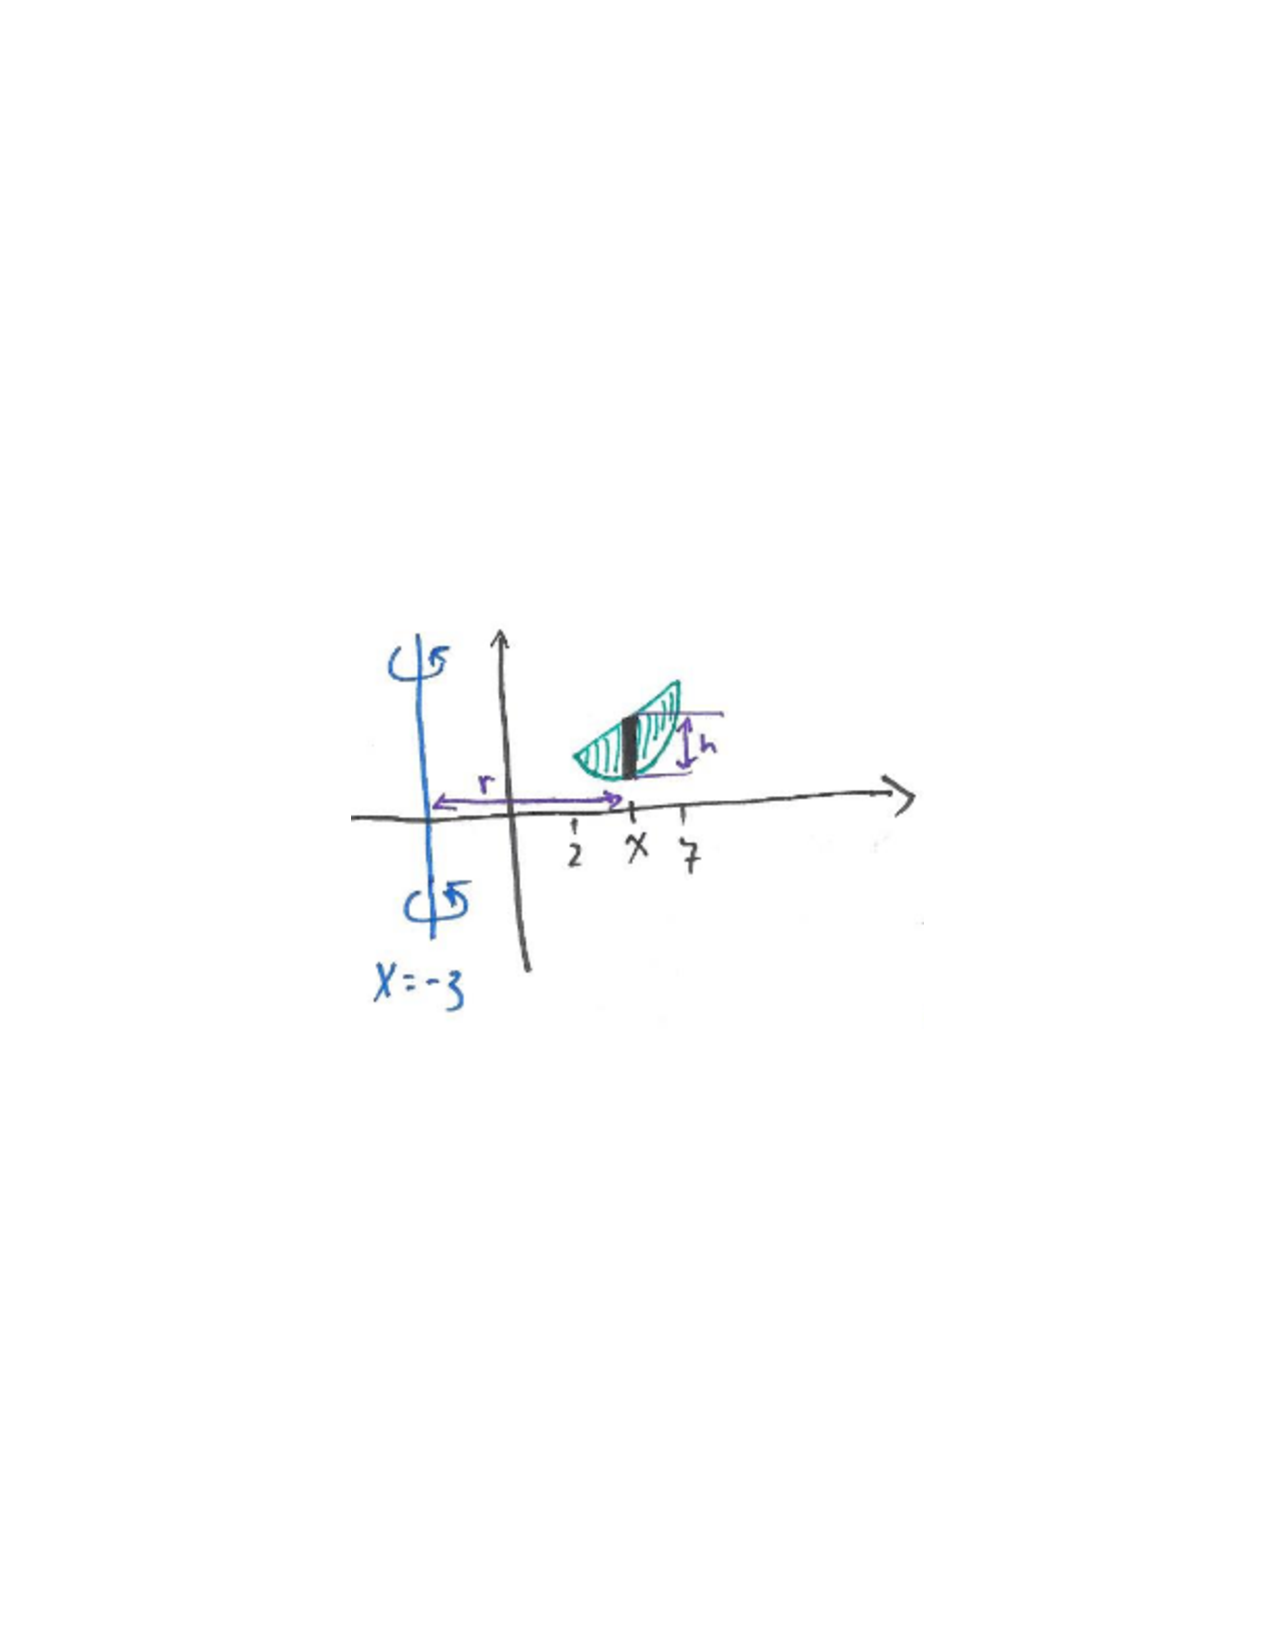
\includegraphics{Figure6-4-10.png}
\end{image}

	
\underline{Washers}:  To use washers, we want slices perpendicular to the axis of revolution.  The axis is $y=-1$ which is a horizontal line, so we want vertical slices.  Therefore, we want to integrate in terms of $x$.  

\begin{image}
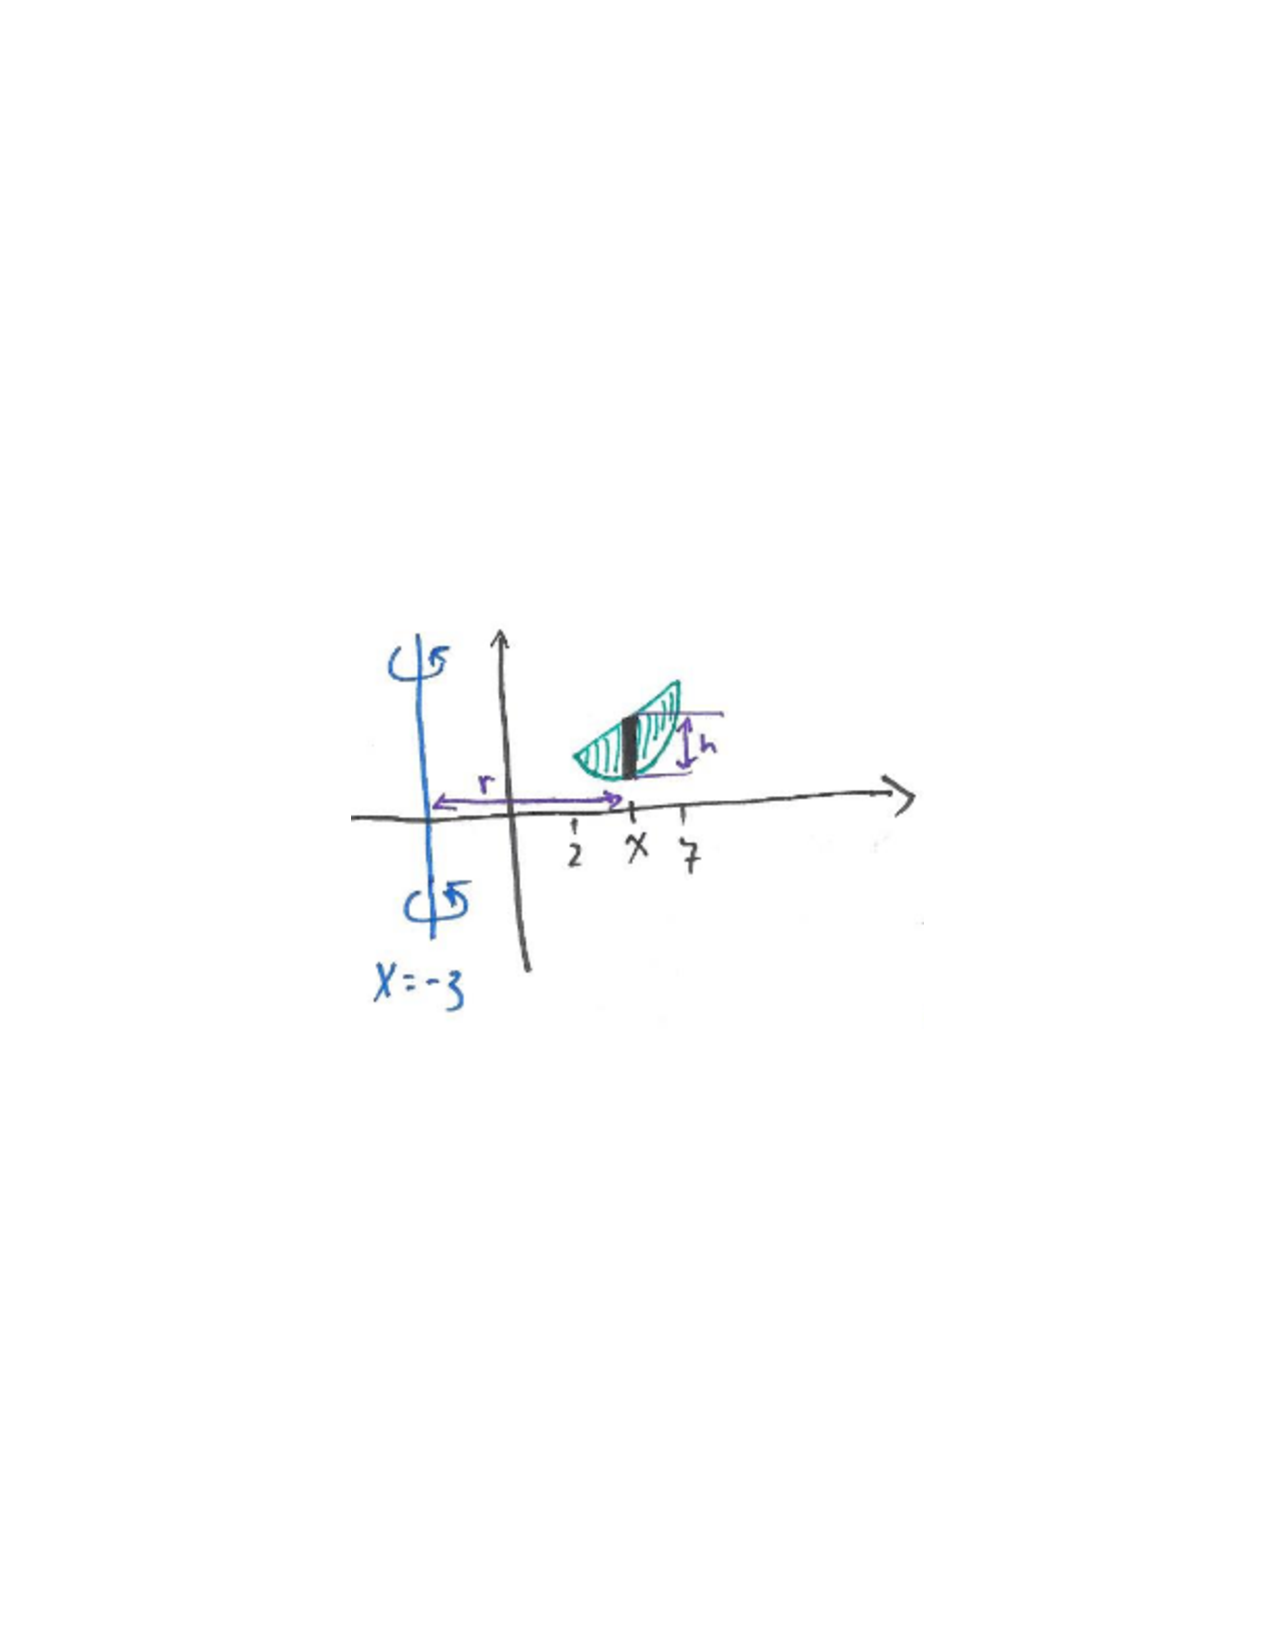
\includegraphics{Figure6-4-11.png}
\end{image}

We can see from the figure that the $x$ values range from 0 to 1.  We have:
\begin{align*}
r_{out} = R(x) &= 2-(-1) = 3\\
r_{in} = r(x) &= (2 -2x) - (-1) = 3 - 2x
\end{align*}

Thus, 
\begin{align*}
V &= \pi \int_0^1 \left( (3)^2 - (3 - 2x)^2 \right) \d x \\
&= \pi \int_0^1 \left( 9 - (9 -12x + 4x^2) \right) \d x \\
&= \pi \int_0^1 \left(- 4x^2+12x ) \right) \d x \\
&= \pi \eval{\frac{-4x^3}{3}+6x^2}_0^1 \\
&= \pi \left(\frac{-4(1)^3}{3}+6(1)^2) \right) - \pi \left(\frac{-4(0)^3}{3}+6(0)^2 \right)\\
&= \pi \frac{14}{3}
\end{align*}

\underline{Shells}:  To use shells, we want slices parallel to the axis of revolution.  The axis is $y=-1$ which is a horizontal line, so we want horizontal slices.  Therefore, we want to integrate in terms of $y$.  We need to solve $y=2-2x$ for $x$.  We get $x=1-\frac{y}{2}$.

\begin{image}
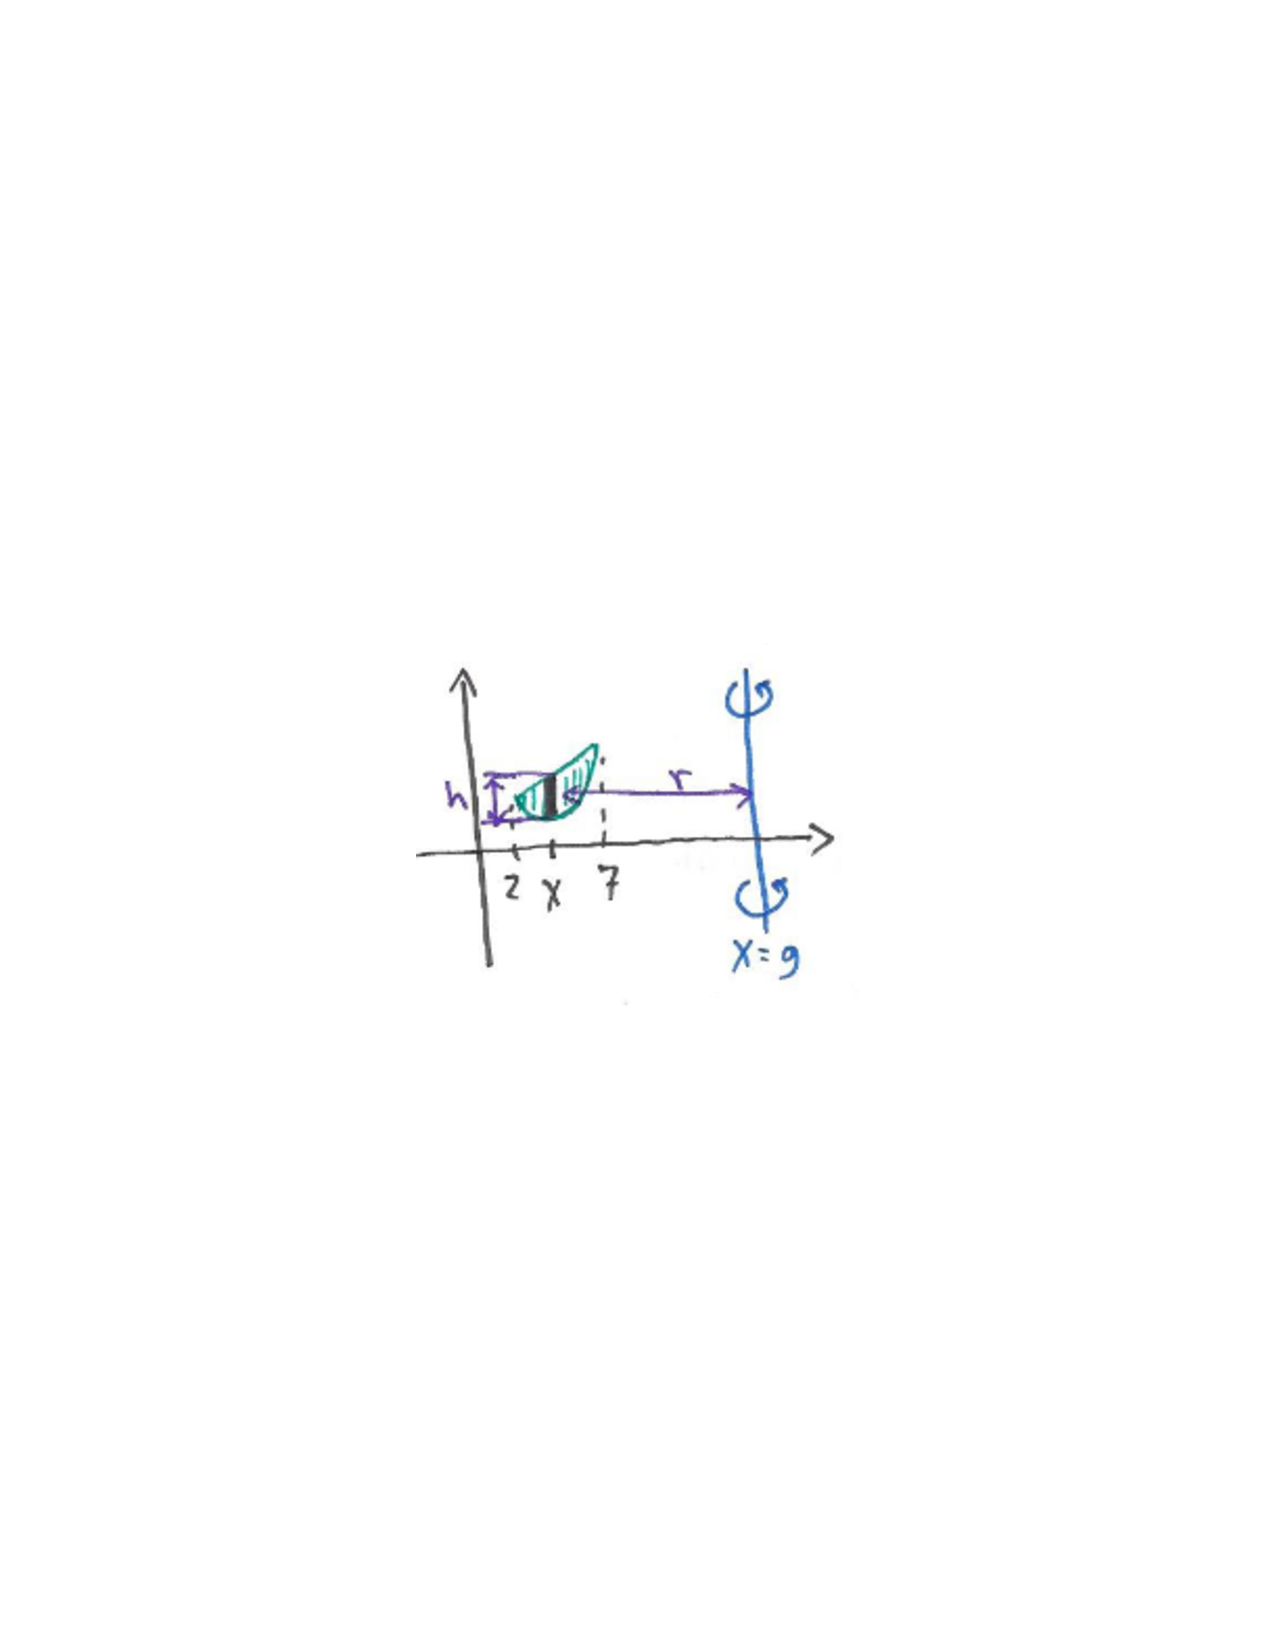
\includegraphics{Figure6-4-12.png}
\end{image}

\begin{align*}
r &= y - (-1) = y+1 \\
h &= 1 - (1-\frac{y}{2}) = 0.5y
\end{align*}

We can see from the figure that $y$ ranges from 0 to 2.

Thus, 
\begin{align*}
V &= 2\pi \int_0^2 \left( rh) \right) \d y \\
&= 2\pi \int_0^2 \left( (y+1)(0.5y) \right) \d y \\
&= \pi \int_0^2 \left( y^2 + y \right) \d y \\
&= \pi \eval{\frac{y^3}{3}+\frac{y^2}{2} }_0^1 \\
&= \pi \left(\frac{(2)^3}{3}+\frac{(2)^2}{2} \right) - \pi \left(\frac{(0)^3}{3}+\frac{(0)^2}{2} \right)\\
&= \pi \frac{14}{3}
\end{align*}

	\end{freeResponse}

\end{problem}


%problem 4
\begin{problem}
Set up an integral that will compute the volume of the solid generated by revolving the region bounded by the curves $y=x^2-6x+13$ (i.e. $x = 3 \pm \sqrt{y-4}$) and $y=3x-1$ about the given axes.  Use the best/easiest method for each problem.

\begin{image}
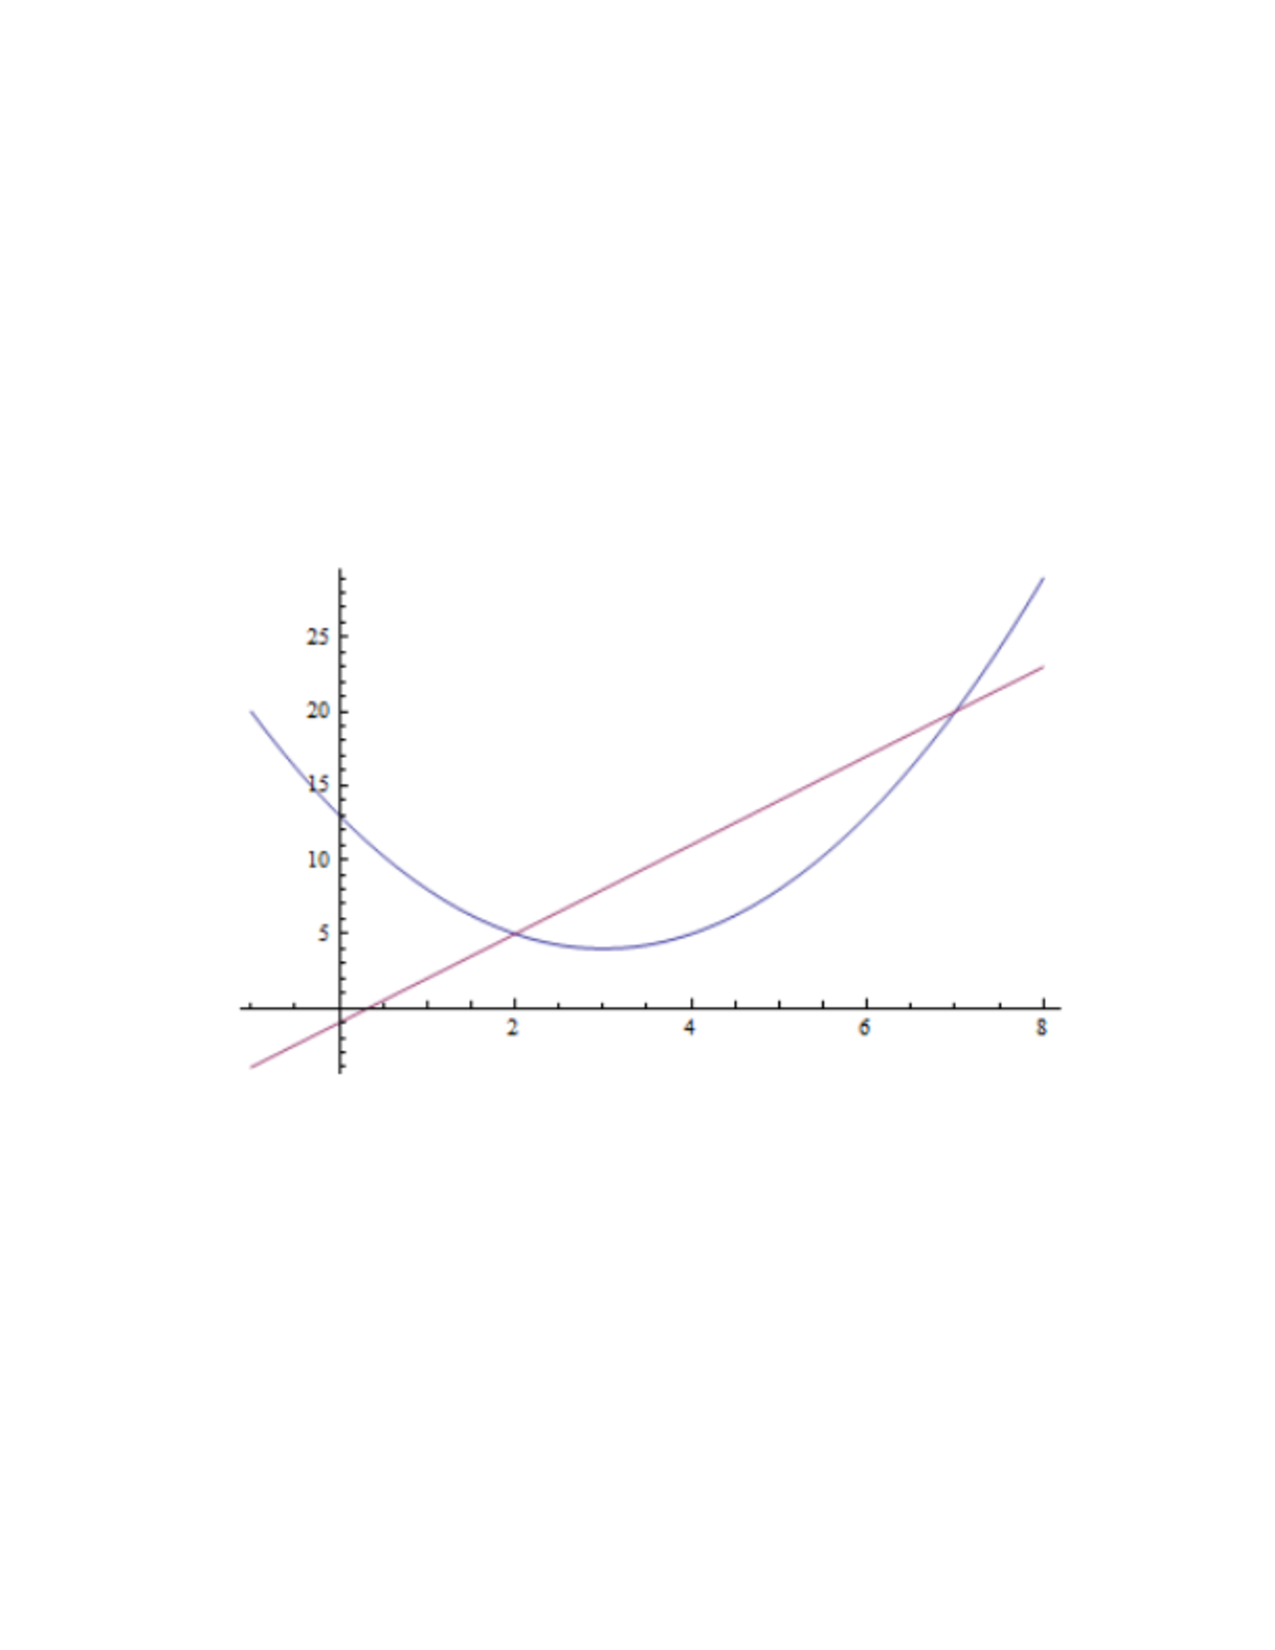
\includegraphics[trim= 170 270 150 280, scale=0.8]{Figure6-4-1.pdf}
\end{image}

	\begin{enumerate}
		\item  the $x$-axis
		\begin{freeResponse}
		First, we need to find the points where the curves intersect
			\begin{align*}
			x^2 - 6x + 13 &= 3x - 1  \\
			x^2 - 9x + 14 &= 0  \\
			(x-2)(x-7) &= 0  \\
			x &= 2, 7  \\
			(2,5&), (7,20).
			\end{align*}
	%	As we will see later, we also need to locate the vertex of the parabola $x^2 - 6x + 13$.  
	%	So we complete the square
	%		\begin{align*}
	%		y &= x^2 - 6x + 13  \\
	%		&= (x^2 - 6x \, {\color{red} + \, 9}) + 13 \, {\color{red} - \, 9}  \\
	%		&= (x-3)^2 + 4.
	%		\end{align*}
	%	So the vertex of the parabola is $(3,4)$.  
		
		\begin{image}
		\includegraphics[scale=0.6]{Figure6-4-1new.png}
		\end{image}
		
		We can see from both the figure and the equations that we would prefer to integrate in terms of $x$.  (If we were to integrate in terms of $y$, we would need two integrals.)  Therefore, our slices will be vertical and perpendicular to the axis of rotation, so we will use washers.\\

		{\bf Washers: }  
		We have that
			\begin{align*}
			r_{out} = R(x) &= 3x-1 \\
			r_{in} = r(x) &= x^2 - 6x +13
			\end{align*}
		and
			\[
			\text{{\color{red} Volume of the region}} = \pi \int_2^7 \left[ (3x-1)^2 - (x^2-6x+13)^2 \right] \d x.
			\]
			
		\begin{image}
		\includegraphics[scale=0.6]{Figure6-4-3new.png}
		\end{image}
		
		%{\bf Shells: }
		%For shells, the cross-sections must be \dfn{parallel} to the axis of rotation.  
		%So here we integrate along the $y$-axis, $5 \leq y \leq 20$.  
		%But we have a problem, namely the ``bottom" of each cross-section changes at $y=5$ due to the shape of the region (see the picture below).
		%So we have two different cases:
			%\begin{enumerate}
			%\item[(1)]  For $4 \leq y \leq 5$
				%\begin{align*}
				%h &= (3+\sqrt{y-1}) - (3-\sqrt{y-1}) = 2\sqrt{y-1}  \\
				%r &= y
				%\end{align*}
			%	
			%\item[(2)]  For $5 \leq y \leq 20$
				%\begin{align*}
				%h &= (3+\sqrt{y-1}) - \left( \frac{1}{3} (y+1) \right)  \\
				%r &= y.
				%\end{align*}
			%\end{enumerate}
		%Thus
			%\[
			%V = \int_4^{20} 2 \pi r h \d y = 2\pi \left[ \int_4^5 y \cdot 2\sqrt{y-1} \d y + \int_5^{20} y \left( (3 + \sqrt{y+1}) - \frac{1}{3}(y+1) \right) \d y \right]
			%\]
		
		%\begin{image}
		%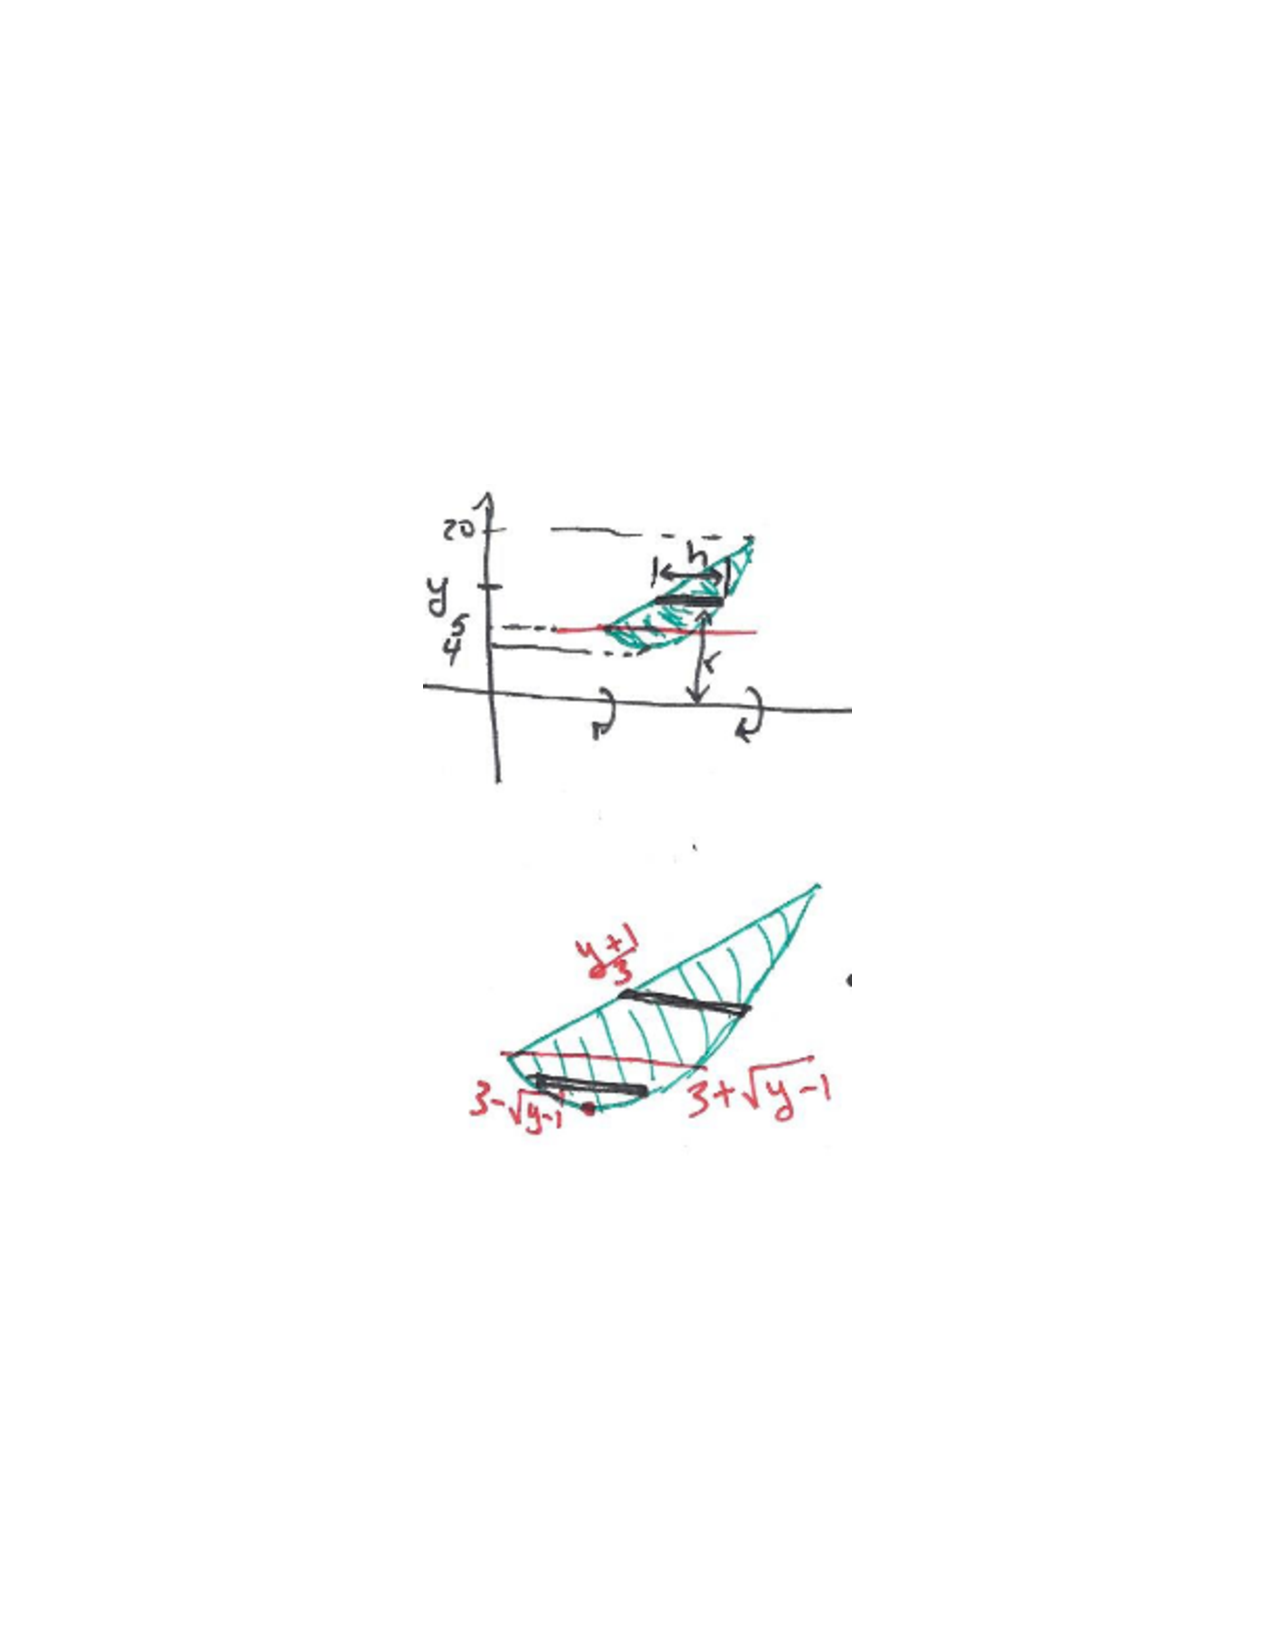
\includegraphics[trim= 200 240 150 240, scale=1]{Figure6-4-4.pdf}
		%\end{image}
		
		%It is pretty clear in this problem that the washer's method was easier than the shell's method.
		\end{freeResponse}
		
		
		
		\item  $y=-4$  
		\begin{freeResponse}
		Our axis is still horizontal so we will use washers again. 
		{\bf Washers: }
		We have that
			\begin{align*}
			r_{out} &= (3x-1) - (-4) = 3x + 3 \\
			r_{in} &= (x^2 - 6x +13) - (-4) = x^2 - 6x + 17
			\end{align*}
		and
			\[
			V = \pi \int_2^7 \left[ (3x+3)^2 - (x^2-6x+17)^2 \right] \d x.
			\]
		
		\begin{image}
		\includegraphics[scale=0.6]{Figure6-4-3new2.png}
		\end{image}
		
		%{\bf Shells: }
		%For shells, the cross-sections must be \dfn{parallel} to the axis of rotation.  
		%So here we integrate along the $y$-axis.
		%Just as before though, the equation determining the bottom of the shell changes at $y=5$.  
		%The height of the shell over the two regions is the same as part (a), but now the radius of the shell is $4+y$.
		%So,
		%	\[
		%	V = 2\pi \left[ \int_4^5 (4+y) \cdot 2\sqrt{y-1} \d y + \int_5^{20} (4+y) \left( (3 + \sqrt{y+1}) - \frac{1}{3}(y+1) \right) \d y \right]
		%	\]
			
		%\begin{image}
		%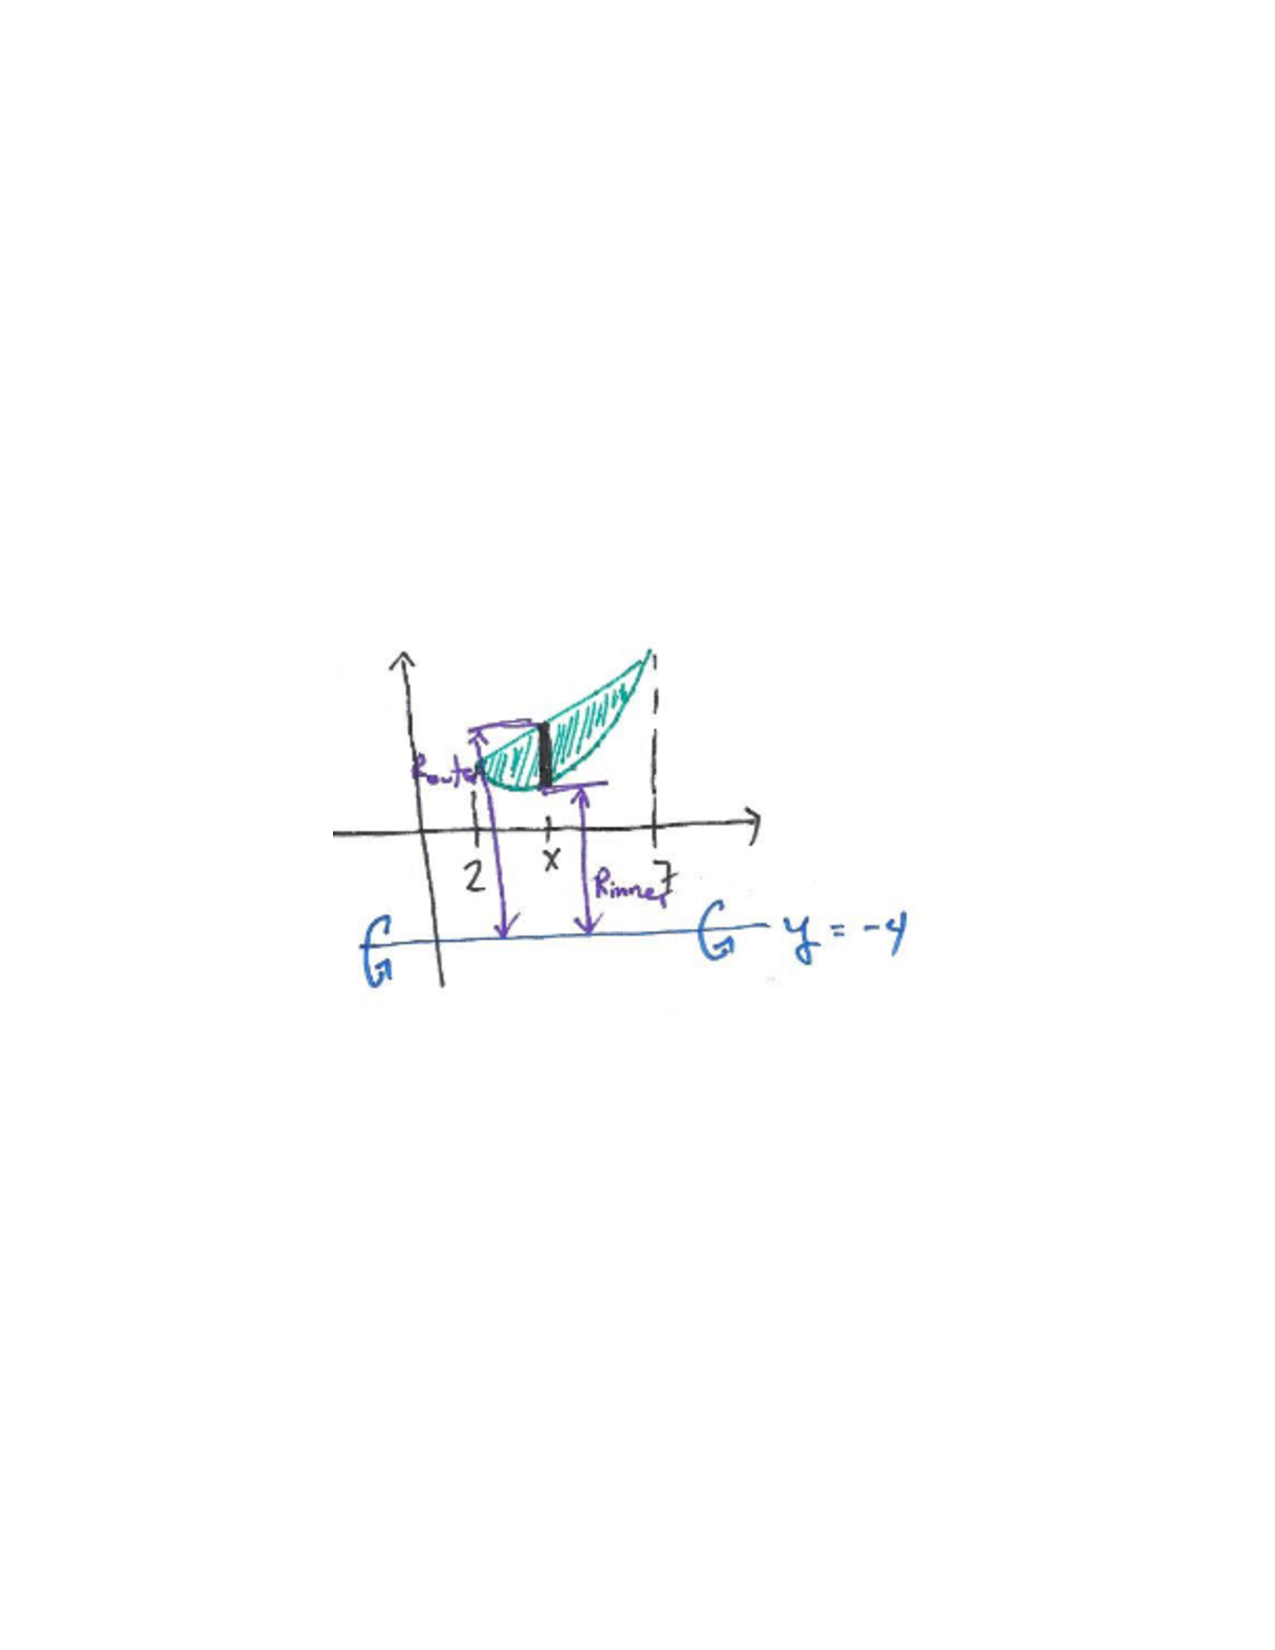
\includegraphics[trim= 150 320 150 310, scale=1]{Figure6-4-5.pdf}
		%\end{image}
		%
		%Again, it is pretty clear that the washer's method was easier than the shell's method for this problem.
		\end{freeResponse}
		
		
		
		\item  $y=22$
		\begin{freeResponse}
		{\bf Washers: }
		Again, since the axis is horizontal and we want to integrate with respect to $x$, we use washers.  The only difference is the axis is above the curve this time.
		We have that
			\begin{align*}
			r_{out} &= 22 -  (x^2 - 6x +13) = -x^2 + 6x + 9 \\
			r_{in} &= 22 -  (3x-1) = -3x + 23
			\end{align*}
		and so
			\[
			V = \pi \int_2^7 \left[ (-x^2+6x+9)^2 - (-3x+23)^2 \right] \d x.
			\]

		%{\bf Shells: }
		%For shells, the cross-sections must be parallel to the axis of rotation.  
		%%So here we integrate along the $y$-axis.
		%Just as before though, the equation determining the bottom of the shell changes at $y=5$.  
		%The height of the shell over the two regions is the same as part (a), but now the radius of each shell is $22-y$.
		%So,
		%	\[
		%	V = 2\pi \left[ \int_4^5 (22-y) \cdot 2\sqrt{y-1} \d y + \int_5^{20} (22-y) \left( (3 + \sqrt{y+1}) - \frac{1}{3}(y+1) \right) \d y \right]
		%	\]
			
		%\begin{image}
		%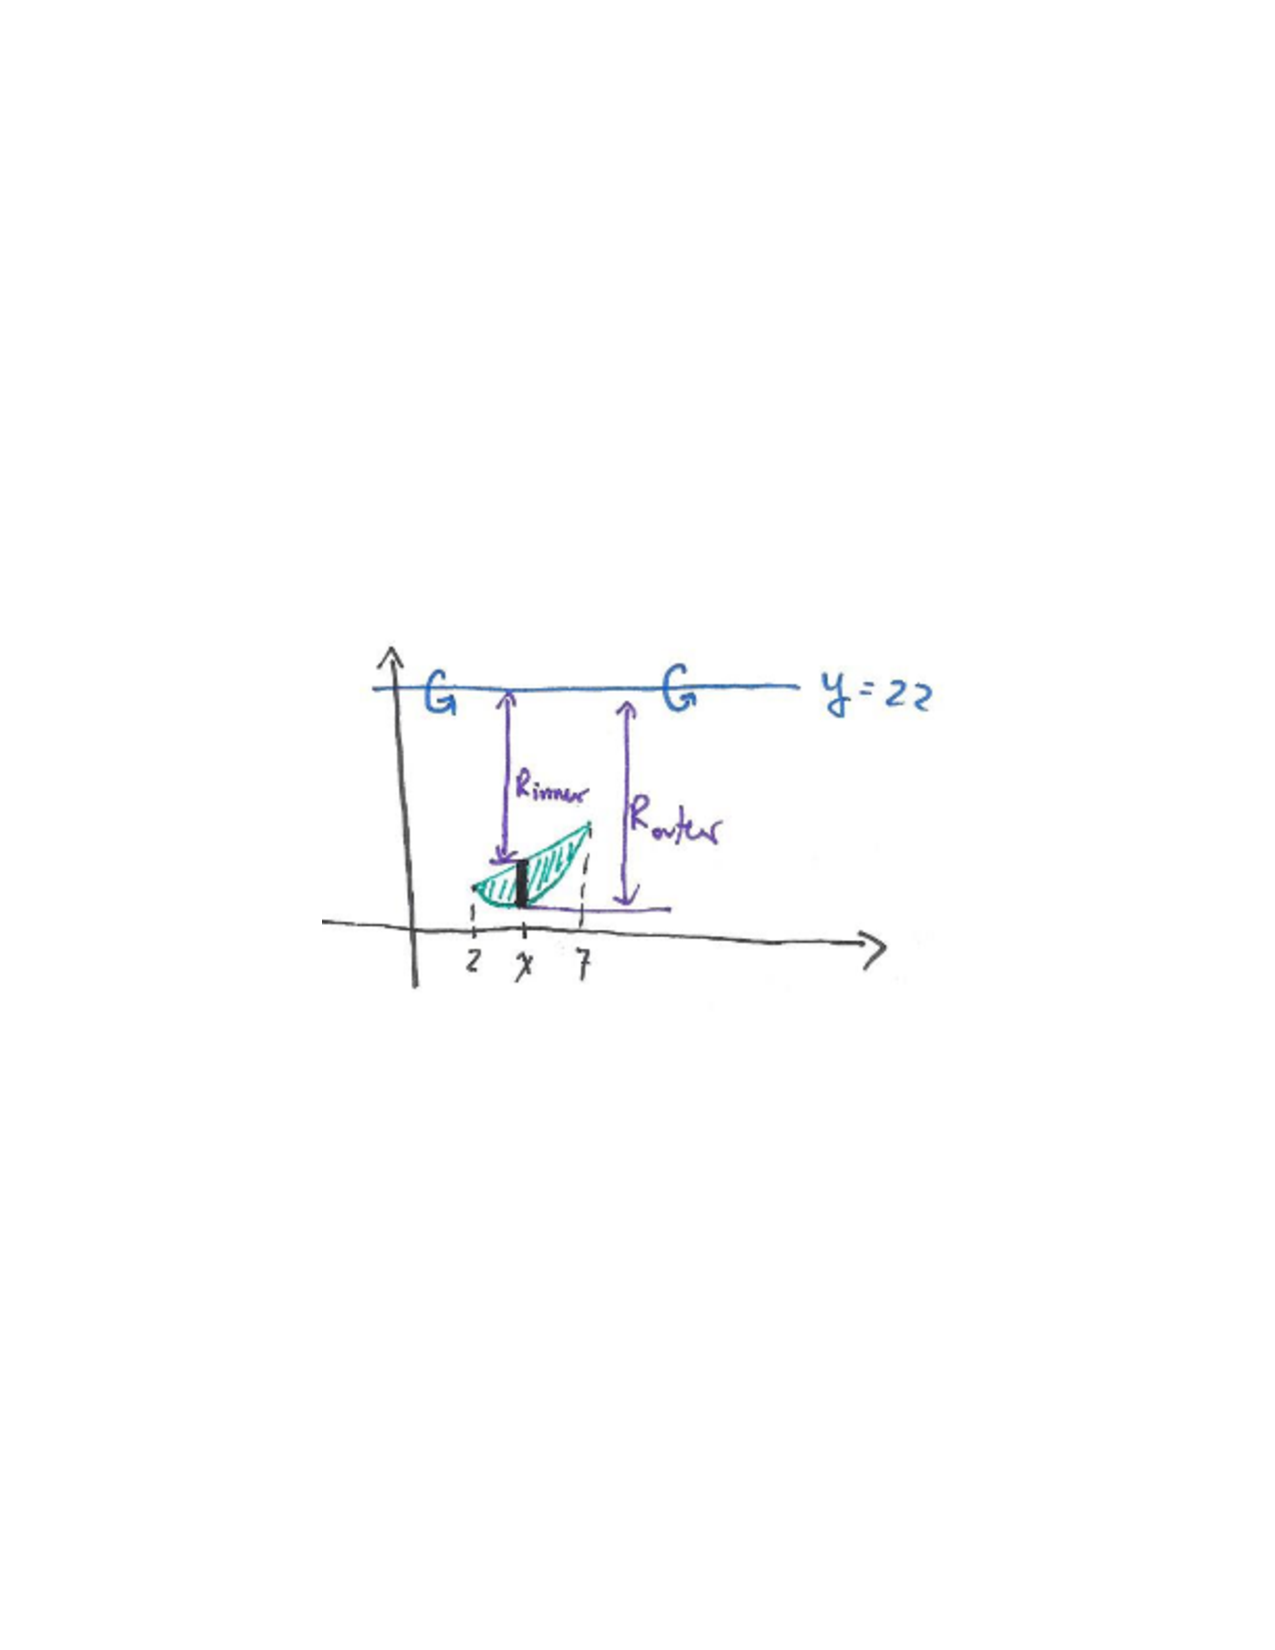
\includegraphics[trim= 150 320 150 310, scale=1]{Figure6-4-6.pdf}
		%\end{image}
		
		%Once again, the washer's method appears to be easier.
		\end{freeResponse}
		
		
		
		\item  the $y$-axis
		\begin{freeResponse}
		%{\bf Washers: }
		%For washers, the cross-sections must be perpendicular to the axis of rotation.  
		%So here we integrate along the $y$-axis (notice the change from the three preceding problems).  
		%Just as in the shells method for the previous three parts, we have to break up our region of integration at $y=5$.  
		%We have the following two cases
		%	\begin{enumerate}
		%	\item[(1)]  for $4 \leq y \leq 5$
		%		\begin{align*}
		%		r_{out} &= 3+\sqrt{y-1} \\
		%		r_{in} &= 3-\sqrt{y-1}
		%		\end{align*}
		%	
		%	\item[(2)]  for $5 \leq y \leq 20$
		%		\begin{align*}
		%		r_{out} &= 3+\sqrt{y-1} \\
		%		r_{in} &= \frac{1}{3}(y+1)
		%		\end{align*}
		%	
		%	\end{enumerate}
		%So,
		%	\[
		%	V = \pi \left[ \int_4^5 \left( \left(3+\sqrt{y-1} \right)^2 - \left(3-\sqrt{y-1}\right)^2 \right) \d y + \int_5^{20} \left( \left( 3+\sqrt{y-1} \right)^2 - \frac{1}{9}(y+1)^2 \right) \d y \right].
		%	\]
			
		%\begin{image}
		%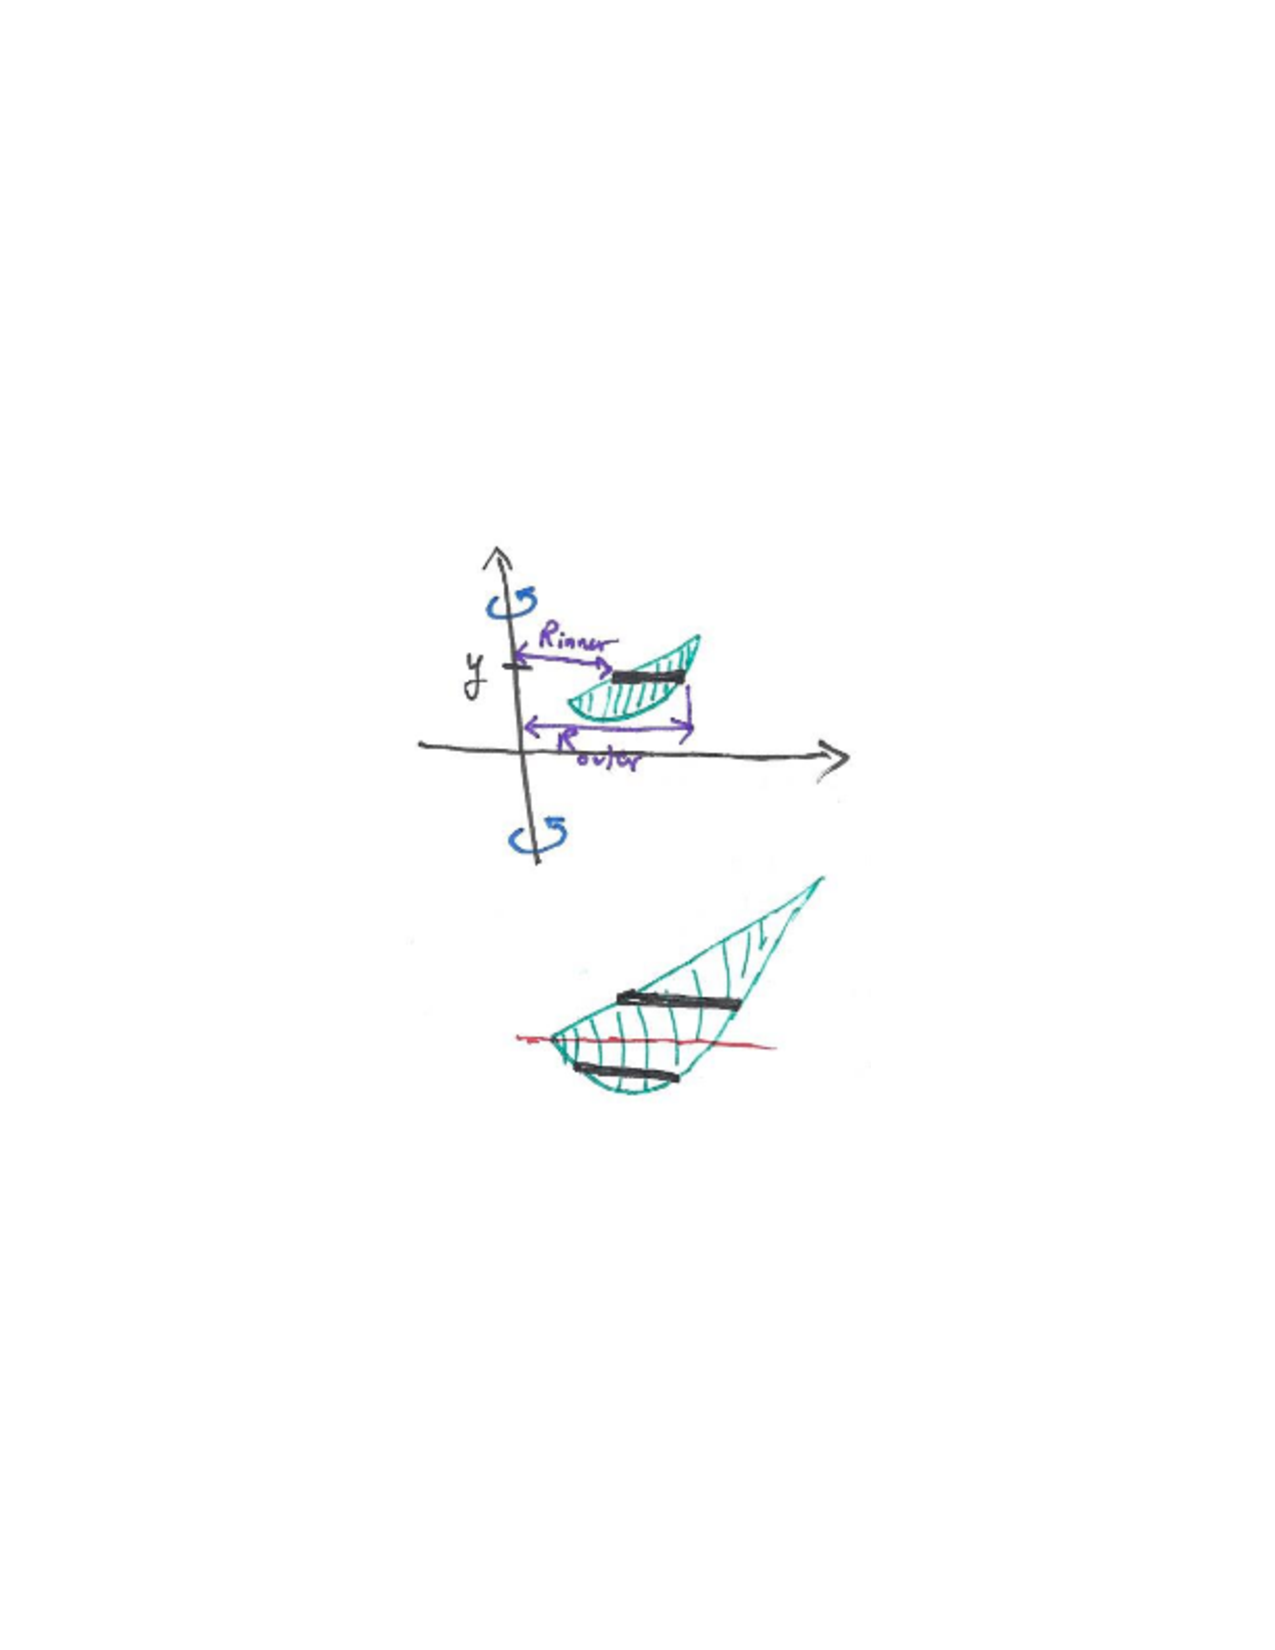
\includegraphics[trim= 150 270 150 270, scale=1]{Figure6-4-7.pdf}
		%\end{image}
		
		Now we have a vertical axis.  Since we want to integrate with respect to $x$ and have parallel slices, we now need to use shells.
		
	      \begin{image}
		\includegraphics[scale=0.6]{Figure6-4-13.png}
		\end{image}

		{\bf Shells: }

			\begin{align*}
			h &= (3x-1) - (x^2-6x+13) = -x^2+9x-14  \\
			r &= x
			\end{align*}
		So,
			\[
			V = 2 \pi \int_2^7 x (-x^2 + 9x - 14) \d x.
			\]

		
		%Now, notice that the shells method was a lot easier.  
		%The key for this region is that you want your cross sections to always be perpendicular to the $x$-axis.
		%That way, the bounds for your parameters do not change over the entire region of integration.
		
		\end{freeResponse}
		
		
		
		\item  $x=-3$
		\begin{freeResponse}
		%{\bf Washers: }
		%For washers, the cross-sections must be perpendicular to the axis of rotation.  
		%So here we integrate along the $y$-axis.
		%Just as in part (d), we need to split the region up into two parts.  
		%But shifting the axis of rotation to $x=-3$ just adds three to all radii.  
		%So
		%	\[
		%	V = \pi \left[ \int_4^5 \left( \left(6+\sqrt{y-1} \right)^2 - \left(6-\sqrt{y-1}\right)^2 \right) \d y \right.
		%	\]
		%	\[
		%	+ \left. \int_5^{20} \left( \left( 6+\sqrt{y-1} \right)^2 - \left( 3 + \frac{1}{3}(y+1) \right)^2 \right) \d y \right].
		%	\]
			
		%\begin{image}
		%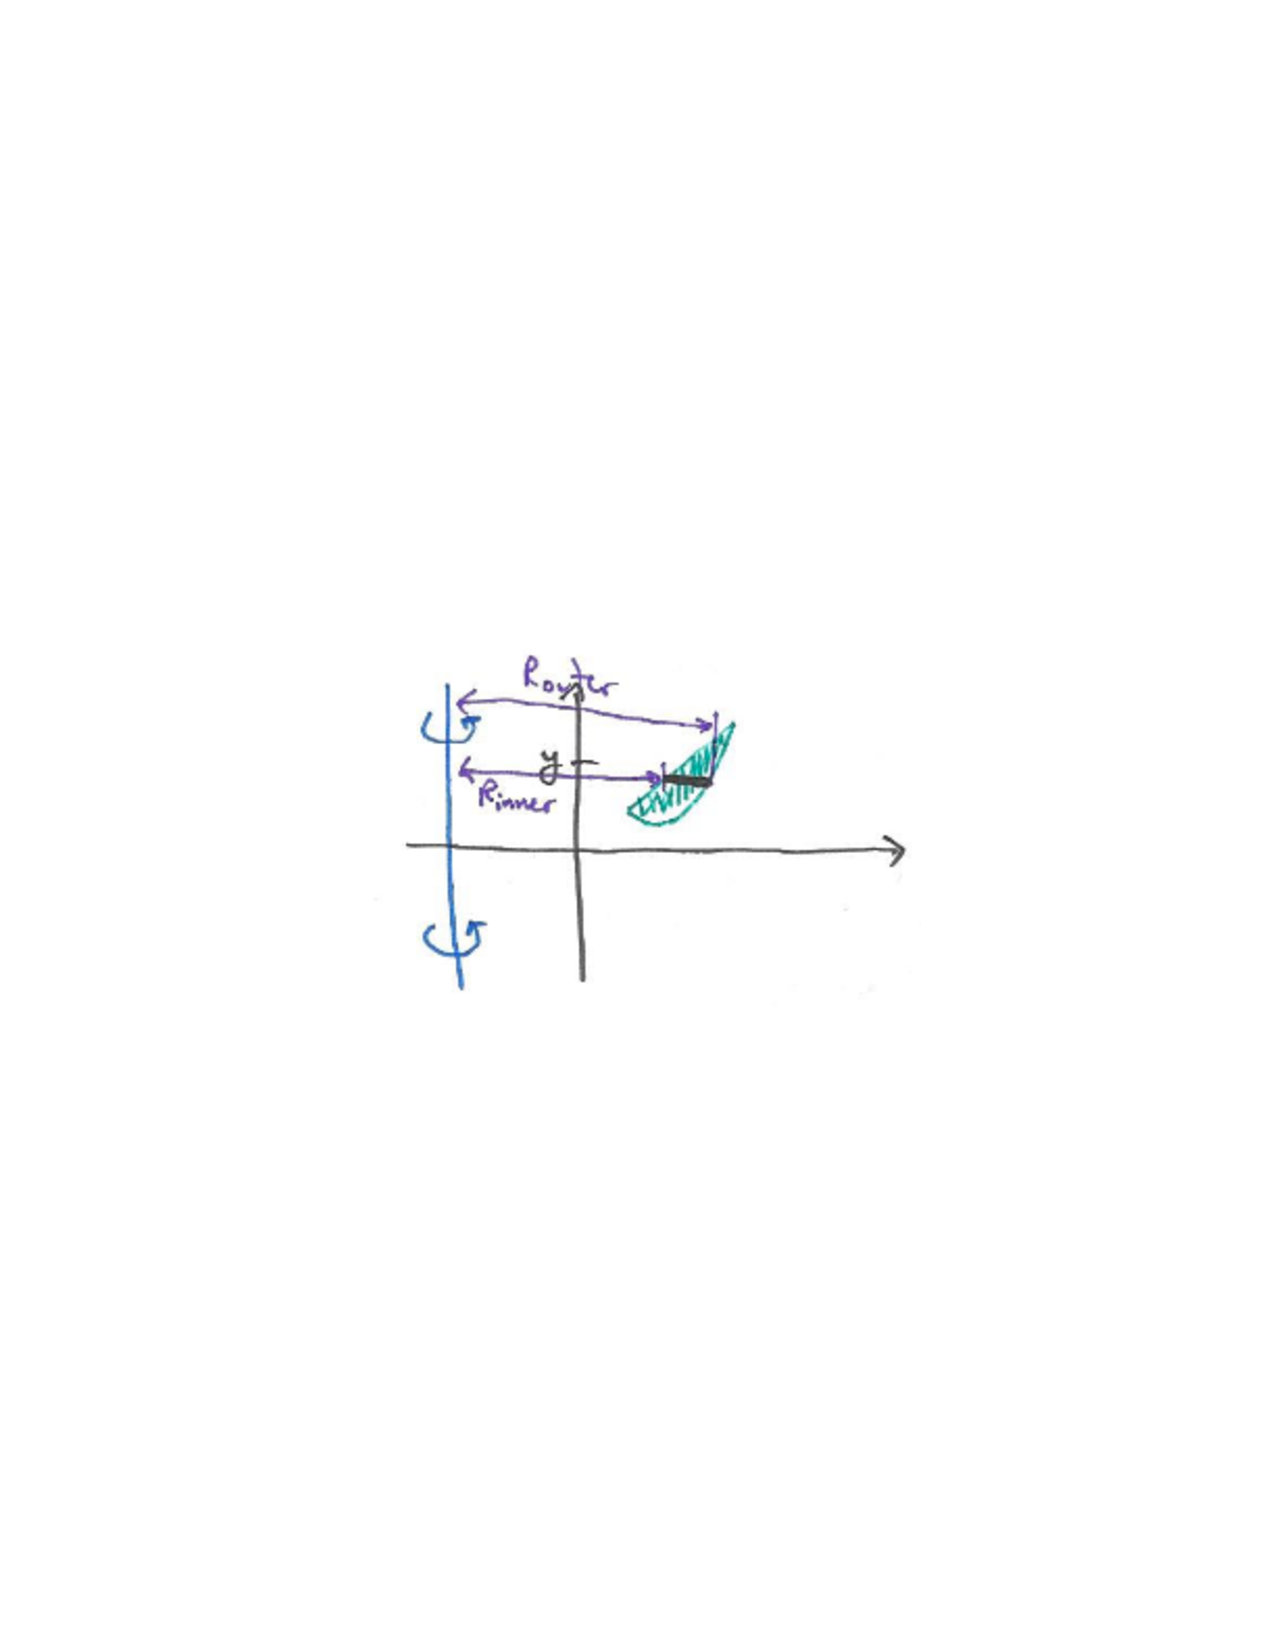
\includegraphics[trim= 150 320 150 310, scale=1]{Figure6-4-9.pdf}
		%\end{image}
		
		Again we have a vertical axis.  Since we want to integrate with respect to $x$ and have parallel slices, we use shells.
		
		{\bf Shells: }
		
		Shifting the axis of rotation to $x=-3$ simply adds three to the radius of the shell, so
			\[
			V = 2 \pi \int_2^7 (3+x) (-x^2 + 9x - 14) \d x.
			\]
			
		%\begin{image}
		%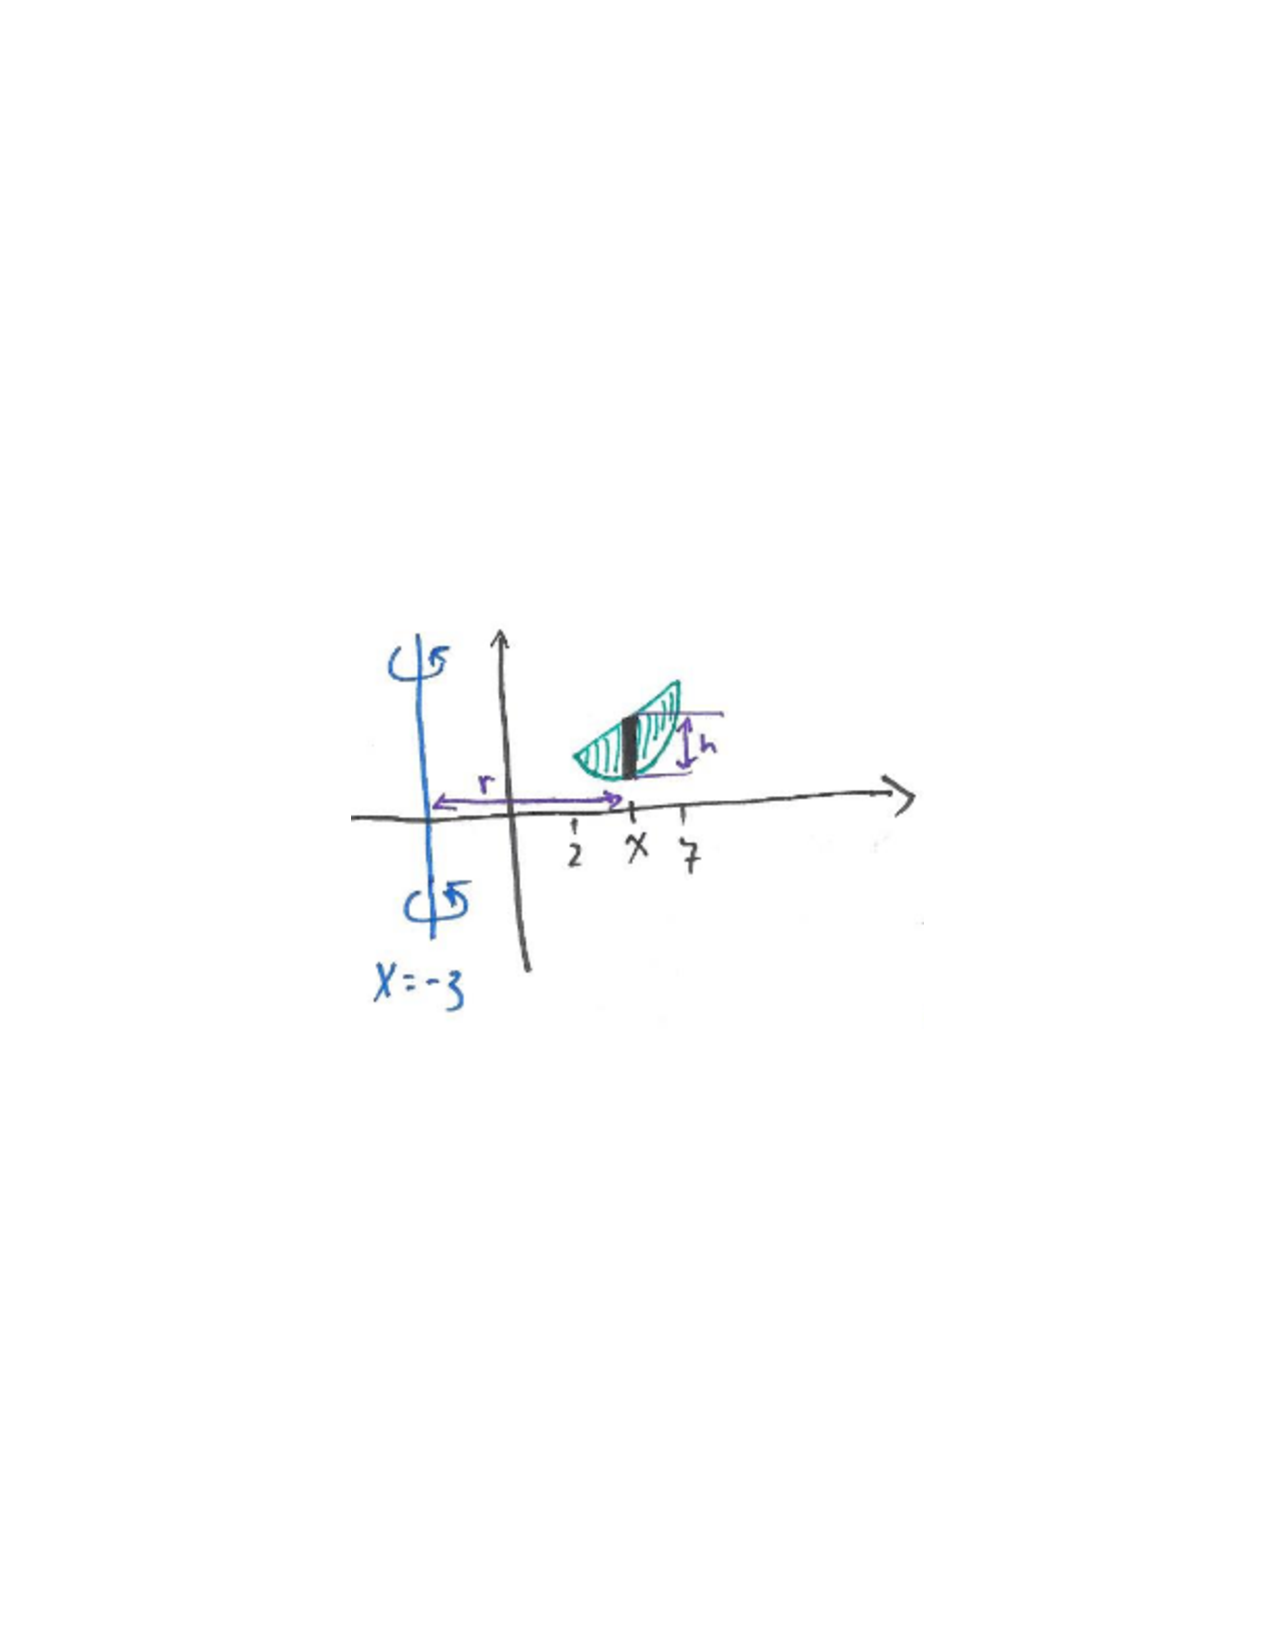
\includegraphics[trim= 150 320 150 310, scale=1]{Figure6-4-10.pdf}
		%\end{image}
		
		%The shells method was simpler.
		\end{freeResponse}
		
		
		
		\item$x=9$
		\begin{freeResponse}
		%{\bf Washers: }
		%For washers, the cross-sections must be perpendicular to the axis of rotation.  
		%So here we integrate along the $y$-axis.
		%Just as in parts (d) and (e), we need to split the region up into two parts.
		%Via the figure below, we compute
		%	\begin{enumerate}
		%	\item[(1)]  for $4 \leq y \leq 5$
		%		\begin{align*}
		%		r_{out} &= 9-\left(3-\sqrt{y-1}\right) = 6+\sqrt{y-1} \\
		%		r_{in} &= 9-\left(3+\sqrt{y-1}\right) = 6-\sqrt{y-1}
		%		\end{align*}
			
		%	\item[(2)]  for $5 \leq y \leq 20$
		%		\begin{align*}
		%		r_{out} &= 9-\left( \frac{1}{3} (y+1) \right)  \\
		%		r_{in} &= 9-\left( 3+\sqrt{y-1} \right) = 6-\sqrt{y-1}
		%		\end{align*}
				
		%	\end{enumerate}
		%So,
		%	\[
		%	V = \pi \left[ \int_4^5 \left( \left(6+\sqrt{y-1} \right)^2 - \left(6-\sqrt{y-1}\right)^2 \right) \d y \right.
		%	\]
		%	\[
		%	+ \left. \int_5^{20} \left( \left( 9 -  \frac{1}{3}(y+1) \right)^2 - \left( 6 - \sqrt{y-1} \right)^2 \right) \d y \right].
		%	\]
			
		%\begin{image}
		%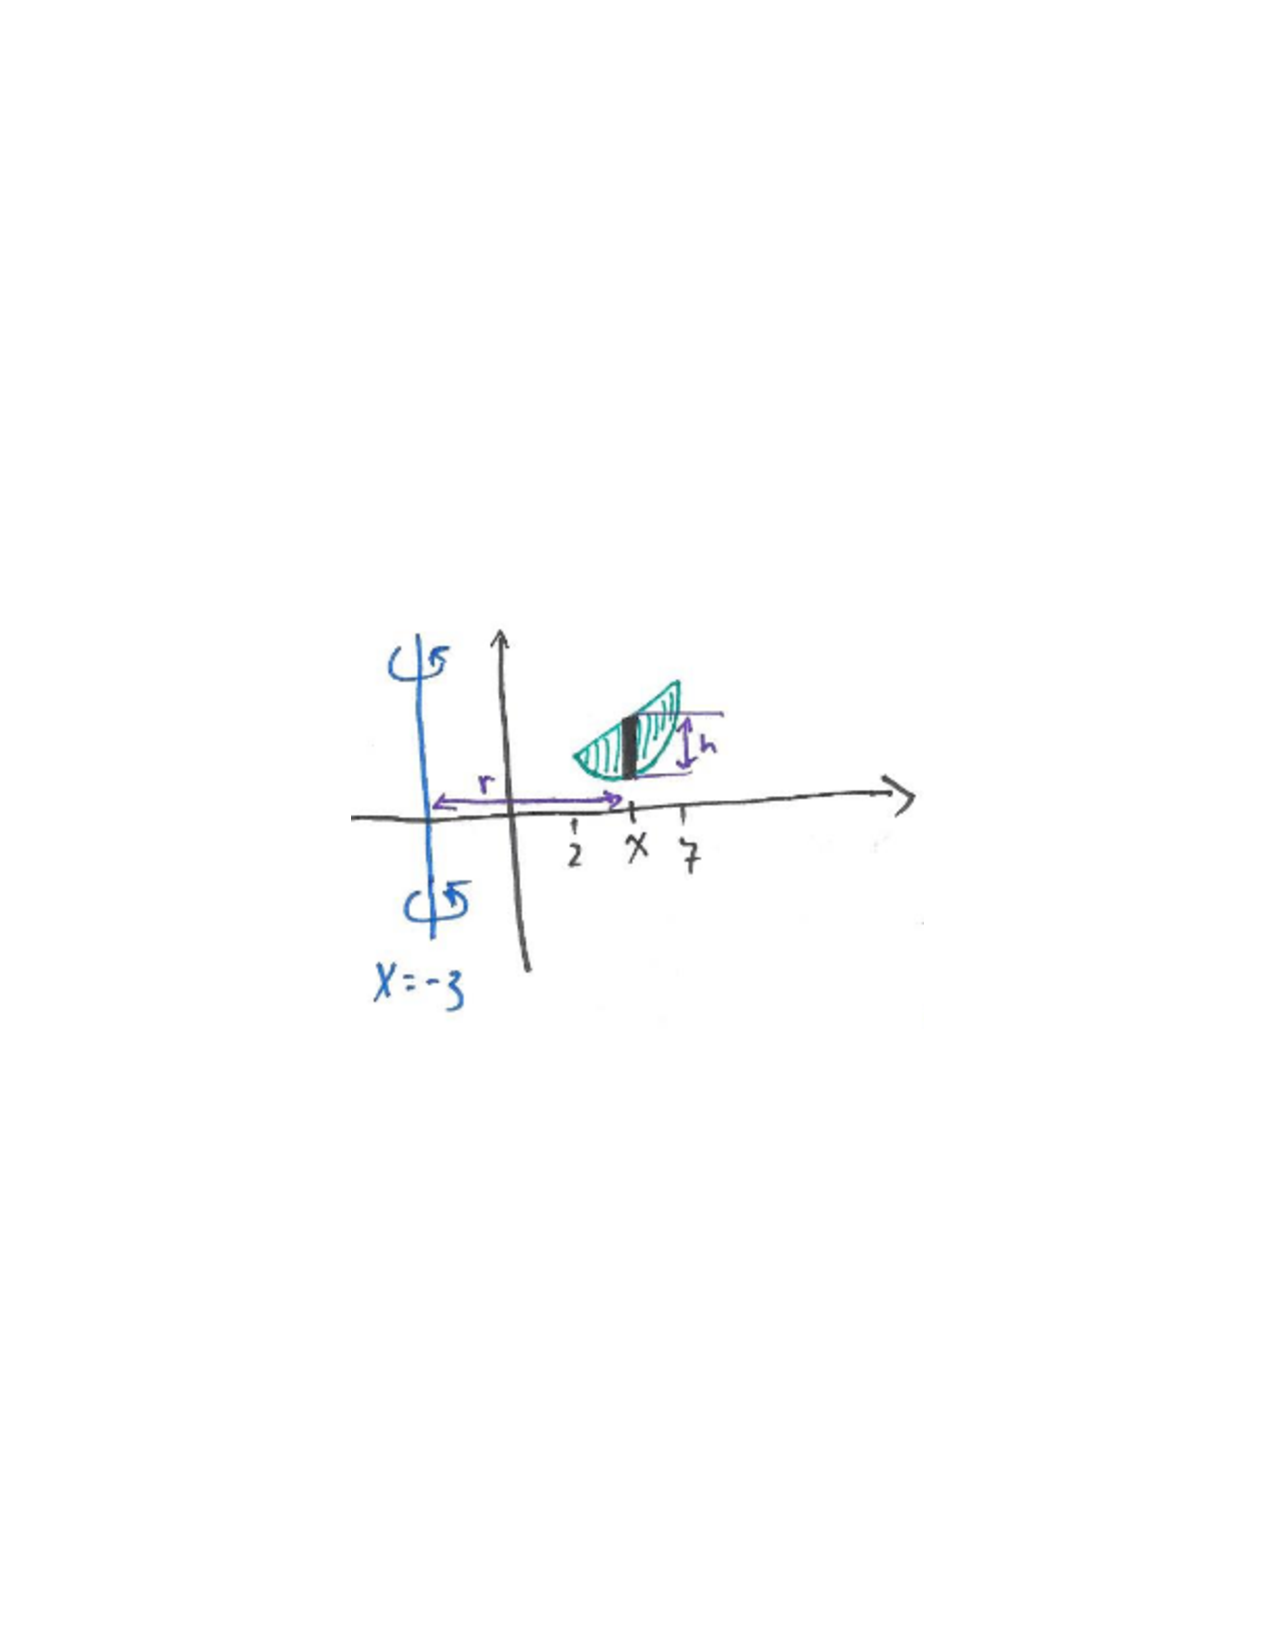
\includegraphics[trim= 150 310 150 300, scale=1]{Figure6-4-11.pdf}
		%\end{image}
		
		
		Again we have a vertical axis.  Since we want to integrate with respect to $x$ and have parallel slices, we use shells.
		
		\begin{image}
		\includegraphics[scale=0.6]{Figure6-4-15.png}
		\end{image}
		
		{\bf Shells: }
		Shifting the axis of rotation to the right 9 units (from part (d)) does not change the height of the cylinder, and the radius changes to $9-x$.
		So
			\[
			V = 2 \pi \int_2^7 (9-x) (-x^2 + 9x - 14) \d x.
			\]
			
		
		
		%Again, the shell method was much simpler.

		\end{freeResponse}
		
	\end{enumerate}
	
\end{problem}

\begin{instructorNotes}
Note that part (a) was on the Recitation \# 3 handout. Remind the students about the solution of part (a). 
For (b)-(e), split these between the groups. Allow time for group work and discussion.   
During the discussion, you might want to talk about all of the ``washer methods" before all of the ``shell methods".  
Be sure that they recognize (by the end) that we slice \dfn{perpendicular} to the axis of revolution in the washer method and \dfn{parallel} to the axis of revolution in the shell method.
\end{instructorNotes}


















	
	
	
	
	
	
	
	
	

	










								
				
				
	














\end{document} 


















